
\section{(More) Understandability Estimators}
\label{sec:proxies}

The correlation of readability formulas as shown in Figure~\ref{fig:bar_corr_clef15} %and~\ref{fig:bar_corr_clef16}
is not strong, without any correlation coefficient being higher than 0.5.
Our next intent is comparing the correlation coefficient of the traditional readability formulas with other methods for understandability estimation, including an evaluation of other humans performing the same task.
For that, we devise and group several methods into semantically related groups which will be following presented.
We summarize all methods in Table~\ref{tab:doc_features}.

%Therefore, what unifies all methods listed in this section is the goal to automatically infer the understandability of a document, in our case, a Web page with medical content.
%For sake of understanding, in Table~\ref{tab:doc_features} we list all the methods used in this chapter to estimate document understandability.
%Note that we divide these estimators into semantically related groups, which are presented below.

\textbf{Traditional Readability Formulas:}
This group contains a large set of traditional readability formulas. Some were mentioned in Section~\ref{sec:related}. A full list can be found in surveys such as Collins-Thompson~\cite{collins2014computational} or Dubay~\cite{dubay04}.

\textbf{Raw Components of Readability Formulas:}
This group comprises the building blocks that make up the traditional readability measures. Some examples include the average number of characters per word or the average number of syllables in a sentence. Words were divided into syllables using the Python package Pyphen \cite{pyphen}.

\textbf{General Medical Vocabularies:}
This group includes methods such as the number of words with a medical prefix or suffix, i.e. beginning or ending with Latin or Greek particles (e.g., amni-, angi-, algia-, arteri-), acronyms or medical vocabularies such as the International Statistical Classification of Diseases and Related Health Problems (ICD), Drugbank and the OpenMedSpel dictionary \cite{openmedspel}.
Acronym list was obtained from ADAM database~\cite{zhou2006}. Methods listed here were matched with documents using a simple keywords matching.

\textbf{Consumer Vocabulary Features:}
NLM MetaMap~\cite{aronson10} was employed to map the content of Web documents to the CHV vocabulary~\cite{zeng06}.
We further use MetaMap options to also filter only concepts identified as symptoms or diseases.
Similar approach is commonly used in the literature \cite{} \mytodo{maybe cite something that is not ours}.
%The CHV dataset (version 20110204) links part of the UMLS concepts, such as “myocardial infarction”, to everyday expressions, “heart attack”.

\textbf{Expert Vocabulary Features:}
As done with CHV, we used MetaMap to map the content of Web documents to MeSH, exploring symptoms and disease concepts separately. 

\textbf{Natural Language:}
This group comprises commonly used metrics in the natural language processing field, such as the ratio of part-of-speech (POS) classes, the number of entities in a text, the sentiment polarity and the ratio of words found in English vocabularies. The Python package NLTK~\cite{nltk} was employed for sentiment analysis and POS tagging. The GNU Aspell~\cite{aspell} dictionary was used as a standard English vocabulary and a stopword list was built by merging the stopword
lists of the Indri~\cite{indri} and Terrier~\cite{terrier} toolkits. 

\textbf{HTML Features:}
The aim of this group is to represent a web page by its HTML content.
We hypothesize that a Web page rich of images or with its content well summarized in tables can potentially ease hard subjects such as medicine. 
We identify a large number of HTML tags in this group with the Python library BeautifulSoap \cite{bs4}.

\textbf{Word Frequency Features:}
Common and known words are usually frequent words, while unknown and obscure words are rare. This idea is implemented in readability formulas such as the Dale-Chall index which uses a list of common words and counts the number of words that fall outside this list~\cite{dale48}.
In this work we model word frequency in a straightforward manner: we sort the frequency of all words in a corpus and normalize the ranking of word frequency such that values close to 100 are attributed to common words and values close to 0 to rare words. 
We explore three different corpora in this work:

\begin{itemize}
\item \underline{Medical Reddit:} Reddit~\cite{reddit} is an Internet forum with a sizable user community which is responsible for generating its content. Any user can start a discussion receiving replies from any other user. This discussion forum is intensively used for health purposes, for example in the Reddit community AskDocs~\cite{redditaskdocs} licensed nursers and doctors (subject to user identity verification) advise help seekers free of charge. We selected six of such communities
    (medical, AskDocs, AskDoctorSmeeee, Health, WomensHealth, Mens\_Health) and downloaded all user interactions using the Python library PRAW~\cite{redditapi}. In total 43,018 discussions were collected.

\item \underline{PubMed Central:} PubMed Central~\cite{pubmed} is an online digital database of freely available full-text biomedical literature playing a similar role to physicians as the ACM Digital Library does to computer scientists. We used in this work the same collection crafted for the TREC Clinical Decision Support Track 2014 and 2015 (TREC-CDS)~\cite{roberts16,trec15} consisting of 733,138 articles. 
 
\item \underline{Medical English Wikipedia:} we filtered articles from a Wikipedia dump~\cite{wikipedia} (May 1st 2017), that contained an Infobox\footnote{A Wikipedia infobox is a template containing structured information that appear on the right of Wikipedia pages to summarize key aspects of concepts} in which at least one of the following words appeared as a property: ICD10, ICD9, DiseasesDB, MeSH, MeSHID, MeshName, MeshNumber, GeneReviewsName, Orphanet, eMedicine, MedlinePlus, drug\_name, Drugs.com, DailyMedID, LOINC.
%Figure~\ref{fig:hyperthermia} illustrates a Wikipedia page that is marked as medical because of its Infobox entries.
This idea was successfully implemented in Soldaini et al.~\cite{soldaini15} and our filtering process resulted in a collection of 11,942 articles. 
Note that this procedure highly favors precision over recall. %\mytodo{In case we need space, I suggest we drop this figure}
\end{itemize}

A summary of the statistics of these three collections is reported in Table~\ref{tab:collection_stats}.
In order to calculate word frequency, we removed words that occur less than 5 times in a corpus.
Finally, unless it is explicitly stated otherwise, we ignore out of vocabulary (OV) words in our calculations,

%\begin{figure}[th!]
%   \centering
%   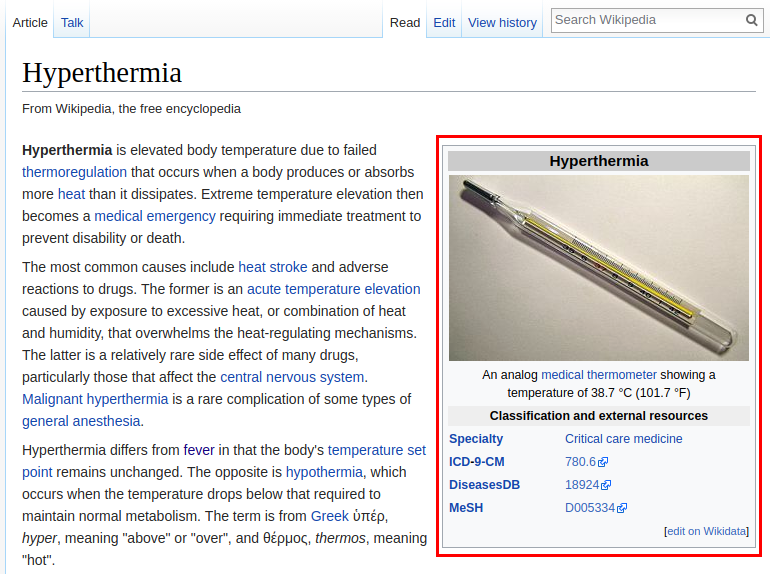
\includegraphics[width=0.50\textwidth]{graphics/hyperthermia}
%    \caption{Wikipedia page on hyperthermia. A rectangular red box identify the Infobox on the right hand side containing entries for Specialty, ICD-9-CM, DiseasesDB and MeSH.}
%    \label{fig:hyperthermia}
%\end{figure}

\begin{table}[!tb]
\centering    
\caption{Statistics for the collections used as background models for understandability estimations.}
\vspace{-0.3cm}
\label{tab:collection_stats}
\resizebox{0.4\textwidth}{!}{
\begin{tabular}{cccc}
\toprule 
\textbf{Statistic} & \textbf{Medical Wikipedia} & \textbf{Medical Reddit} & \textbf{PubMed Central}\tabularnewline
\midrule 
\textbf{Number of Docs.} & 11,868 & 43,019 & 733,191\tabularnewline
\textbf{Number of Words} & 10,655,572 & 11,978,447 & 144,024,976\tabularnewline
\textbf{Number of Unique Words} & 467,650 & 317,106 & 2,933,167\tabularnewline
\textbf{Avg. Words per Doc.} & 898.90 $\pm$ 1351.76 & 278.45 $\pm$ 359.70  & 227.22 $\pm$ 270.44 \tabularnewline
\textbf{Avg. Char per Doc.} & 5107.81 $\pm$ 7618.57  & 1258.44 $\pm$ 1659.96  & 1309.11 $\pm$ 1447.31 \tabularnewline
\textbf{Avg. Char per Word} & 5.68 $\pm$ 3.75  & 4.52 $\pm$ 3.52 &  5.76 $\pm$ 3.51 \tabularnewline
\bottomrule
\end{tabular}
} % End of resizebox
\vspace{-8pt}
\end{table}


\textbf{Machine Learning on Text - Regressors and Classifiers:}
In a recent survey, Kevin Collins-Thompson reports that the future of understandability estimation relies on Machine Learning~\cite{collins2014computational}.
A challenge in using Machine Learning in this task is defining the background corpora used as training set.
A possible setup for our work could have used CLEF 2015 assessments to learn a model for CLEF 2016 and vice-versa, but instead, we opt for a 
more reusable solution for the medical/health domain. 
We employed the three datasets described in Table~\ref{tab:collection_stats} and assume different labels according to the average difficulty of documents in these collections:

\begin{itemize}
    \item Medical Reddit (label 1): Documents in this collection are expected to be written in a colloquial style, and thus the easiest to understand. All the conversations are in fact explicitly directed to assist inexpert health consumers;
    \item Medical English Wikipedia (label 2): Documents in this collection are expected to be less formal than scientific articles, but more formal than a Web forum like Reddit;
    \item PubMed Central (label 3): Documents from this collection are expected to be written in a highly formal style, as the target audience here are physicians, nursers and researchers in the biomedical domain.
\end{itemize}

Models were trained on a Latent Semantic Analysis (LSA) empirically set to have ten dimension based on word counts in documents in these three collections.
We model two different tasks: a classification one and a regression task.
Different labels for the regression could be employed, for example, a label 6 to PubMed Central documents would emphasize that these documents are explicitly made for expert users, being 3 times harder than Wikipedia ones. We did not explore the effects of different labels in this work, it is left as future work.

\begin{table*}[tb]
\caption{Metrics used as understandability proxies; $\star$: raw values are used. $\diamondsuit$: values normalised by number of words in a documents are used. $\dagger$: values normalised by number of sentences in a document are used.}
\label{tab:doc_features}
\resizebox{1.\textwidth}{!}{
\begin{tabular}{llcll}
\cline{1-2} \cline{4-5} 
\textbf{Group} & \textbf{Metric} & \multirow{29}{*}{} & \textbf{Group} & \textbf{Metric}\tabularnewline
\cline{1-2} \cline{4-5} 
\multirow{8}{*}{\textbf{Traditional Readability Formulas}} & Automated Readability Index (ARI) \cite{ari67} &  & \multirow{26}{*}{\textbf{HTML Features}} & \# of Abbr tags\tabularnewline
 & Coleman-Liau Index (CLI) \cite{cli75} &  &  & \# of A tags\tabularnewline
 & Dale Chall Index (DCI) \cite{dale48} &  &  & \# of Blockquote tags\tabularnewline
 & Flesch-Kincaid Grade Level (FKGL) \cite{flesch75} &  &  & \# of Bold tags\tabularnewline
 & Flesch Reading Ease (FRE) \cite{flesch75} &  &  & \# of Cite tags\tabularnewline
 & Gunning Fog Index (GFI) \cite{gunning52} &  &  & \# of Div tags\tabularnewline
 & Lasbarhetsindex (LIX) \cite{lix} &  &  & \# of Forms tags\tabularnewline
 & Simple Measure of Gobbledygook (SMOG) \cite{smog69} &  &  & \# of H1 tags\tabularnewline
\cline{1-2} 
\multirow{10}{*}{\textbf{\makecell{\kern-2.8emRaw Components \\of Readability Measures}}} & \# of Characters $^{\star\diamondsuit\dagger}$ &  &  & \# of H2 tags\tabularnewline
 & \# of Words $^{\star\dagger}$ &  &  & \# of H3 tags\tabularnewline
 & \# of Sentences {$^{\star\diamondsuit}$} &  &  & \# of H4 tags\tabularnewline
 & \# of Difficult Words (Dale Chall list \cite{dale48})
$^{\star\diamondsuit\dagger}$ &  &  & \# of H5 tags\tabularnewline
 & \# of Words Longer than 4 chars $^{\star\diamondsuit\dagger}$ &  &  & \# of H6 tags\tabularnewline
 & \# of Words Longer than 6 chars $^{\star\diamondsuit\dagger}$ &  &  & \# of Hs (any H above)\tabularnewline
 & \# of Words Longer than 10 chars $^{\star\diamondsuit\dagger}$ &  &  & \# of Img tags\tabularnewline
 & \# of Words Longer than 13 chars $^{\star\diamondsuit\dagger}$ &  &  & \# of Input tags\tabularnewline
 & \# of Number of Syllables $^{\star\diamondsuit\dagger}$ &  &  & \# of Link tags\tabularnewline
 & \# of Polysyllable Words (>3 Syllables) $^{\star\diamondsuit\dagger}$ &  &  & \# of DL tags\tabularnewline
\cline{1-2} 
\multirow{6}{*}{\textbf{Medical Vocabularies}} & \# of Words with Medical Prefix $^{\star\diamondsuit\dagger}$ &  &  & \# of UL tags\tabularnewline
 & \# of Words with Medical Suffix $^{\star\diamondsuit\dagger}$ &  &  & \# of OL tags\tabularnewline
 & \# of Acronyms $^{\star\diamondsuit\dagger}$ &  &  & \# of List (DL + UL + OL)\tabularnewline
 & \# of ICD Concepts $^{\star\diamondsuit\dagger}$ &  &  & \# of Q tags\tabularnewline
 & \# of Drugbank $^{\star\diamondsuit\dagger}$ &  &  & \# of Scripts tags\tabularnewline
 & \# of Words in medical dict. (OpenMedSpel) $^{\star\diamondsuit\dagger}$ &  &  & \# of Spans tags\tabularnewline
\cline{1-2} 
    \multirow{6}{*}{\textbf{\makecell{\kern-2.5emConsumer Health\\ Vocabulary (CHV) \cite{zeng06} \\ \kern-6.2emFeatures}}} & CHV Mean Score for all Concepts $^{\star\diamondsuit\dagger}$ &  &  & \# of Table tags\tabularnewline
 & \# of CHV Concepts $^{\star\diamondsuit\dagger}$ &  &  & \# of P tags\tabularnewline
\cline{4-5} 
 & CHV Mean Score for Symptom Concepts $^{\star\diamondsuit\dagger}$ &  & \multirow{20}{*}{\textbf{Word Frequency}} & 25th percentil English Wikipedia\tabularnewline
 & \# of CHV Symptom Concepts $^{\star\diamondsuit\dagger}$ &  &  & 50th percentil English Wikipedia\tabularnewline
 & CHV Mean Score for Disease Concepts $^{\star\diamondsuit\dagger}$ &  &  & 75th percentil English Wikipedia\tabularnewline
 & \# of CHV Disease Concepts $^{\star\diamondsuit\dagger}$ &  &  & Mean Rank English Wikipedia\tabularnewline
\cline{1-2} 
\multirow{6}{*}{\textbf{\makecell{\kern-0.3emMedical Subject\\ Headers (MeSH)}}} & \# of MeSH Concepts $^{\star\diamondsuit\dagger}$ &  &  & Mean Rank English Wikipedia - Includes OV\tabularnewline
 & Average Tree of MeSH Concepts $^{\star\diamondsuit\dagger}$ &  &  & 25th percentil Medical Reddit\tabularnewline
 & \# of MeSH Symptom Concepts $^{\star\diamondsuit\dagger}$ &  &  & 50th percentil Medical Reddit\tabularnewline
 & Average Tree of MeSH Symptom Concepts $^{\star\diamondsuit\dagger}$ &  &  & 75th percentil Medical Reddit\tabularnewline
 & \# of MeSH Disease Concepts $^{\star\diamondsuit\dagger}$ &  &  & Mean Rank Medical Reddit\tabularnewline
 & Average Tree of MeSH Disease Concepts $^{\star\diamondsuit\dagger}$ &  &  & Mean Rank Medical Reddit ncludelude OV\tabularnewline
\cline{1-2} 
\multirow{20}{*}{\textbf{Natural Language}} & Positive Words $^{\star\diamondsuit\dagger}$ &  &  & 25th percentil Pubmed\tabularnewline
 & Negative Words $^{\star\diamondsuit\dagger}$ &  &  & 50th percentil Pubmed\tabularnewline
 & Neutral Words $^{\star\diamondsuit\dagger}$ &  &  & 75th percentil Pubmed\tabularnewline
 & \# of verbs $^{\star\diamondsuit\dagger}$ &  &  & Mean Rank Pubmed\tabularnewline
 & \# of nouns $^{\star\diamondsuit\dagger}$ &  &  &  Mean Rank Pubmed - Includes OV\tabularnewline
 & \# of pronouns $^{\star\diamondsuit\dagger}$ &  &  & 25th p. Wikipedia+Reddit+Pubmed  \tabularnewline
 & \# of adjectives $^{\star\diamondsuit\dagger}$ &  &  & 50th p. Wikipedia+Reddit+Pubmed \tabularnewline
 & \# of adverbs $^{\star\diamondsuit\dagger}$ &  &  & 75th p. Wikipedia+Reddit+Pubmed \tabularnewline
 & \# of adpositions $^{\star\diamondsuit\dagger}$ &  &  & Mean R. Wiki.+Reddit+Pubmed \tabularnewline 
 & \# of conjunctions $^{\star\diamondsuit\dagger}$ & &  & Mean R. Wiki.+Reddit+Pubmed - w. OV \tabularnewline
\cline{4-5} 
 & \# of determiners $^{\star\diamondsuit\dagger}$ & & \multirow{5}{*}{\textbf{Regressor}} & Linear Regressor\tabularnewline  
 & \# of cardinal numbers $^{\star\diamondsuit\dagger}$ &  &  & Gradient Boosting Regressor\tabularnewline
 & \# of particles or other function words $^{\star\diamondsuit\dagger}$ &  &  & Multi-layer Perceptron Regressor\tabularnewline
 & \# of other POS (foreign words, typos) $^{\star\diamondsuit\dagger}$ &  &  & Random Forest Regressor\tabularnewline
 & \# of punctuation $^{\star\diamondsuit\dagger}$ &  &  & Support Vector Machine Regressor\tabularnewline
\cline{4-5} 
 & Height of part-of-speech parser tree $^{\star\diamondsuit\dagger}$ &  &  \multirow{6}{*}{\textbf{Classifier}} & Logistic Regression\tabularnewline
 & \# of Entities $^{\star\diamondsuit\dagger}$ &  &  & Gradient Boosting Classifier\tabularnewline
 & \# of Stopwords $^{\star\diamondsuit\dagger}$ &  &  & Multinomial Naive Bayes\tabularnewline
 & \# of words not found in Aspell Eng. dict. $^{\star\diamondsuit\dagger}$ &  &  & Multi-layer Perceptron Classifier\tabularnewline
 &  &  &  & Random Forest Classifier\tabularnewline
 &  &  &  & Support Vector Machine Classifier\tabularnewline
\cline{1-2} \cline{4-5} 
\end{tabular}
}
\end{table*}



